Verify all your solutions using arduino.
\begin{enumerate}[label=\arabic*.,ref=\theenumi]
	\item 		Obtain the minimal form for the Boolean expression
\hfill (CBSE 2013)
\label{prob:2013/d/6/d}
		\begin{align*}
%\label{eq:2013/d/6/d}
H(P,Q,R,S)=\sum(0,1,2,3,5,7,8,9,10,14,15)
		\end{align*}
	\item Write the POS form for the function $G$ shown in 
\tabref{tab:2013/c/6/d}.
\hfill (CBSE 2013)
\label{prob:2013/c/6/d}
		\begin{table}[H]
			\centering
			%\resizebox{\columnwidth}{!}
			\caption{}
\label{tab:2013/c/6/d}
 \end{table}
	\item Reduce the following Boolean Expression to its simplest form using K-Map.
\label{prob:2015-1/c/6/d}
		\begin{align*}
%\label{eq:2015-1/c/6/d}
			F(X,Y,Z,W)=(0,1,4,5,6,7,8,9,11,15)
		\end{align*}
\hfill (CBSE 2015)
	\item 
\label{prob:2015/c/6/d}
		Reduce the following Boolean Expression to its simplest form using K-map.

\hfill (CBSE 2015)
		\begin{align*}
%\label{eq:2015/c/6/d}
F(X,Y,Z,W)= \sum (0,1,6,8,9,10,11,12,15)
		\end{align*}
	\item Reduce the following Boolean Expression to its simplest form using K-map.
\label{prob:2016/c/6/d}
		\begin{align*}
%\label{eq:2016/c/6/d}
			F(X,Y,Z,W)= \sum(2,6,7,8,9,10,11,13,14,15)
		\end{align*}
\hfill (CBSE 2016)
	\item Derive a Canonical POS expression for a Boolean function  $F$, represented in 
\tabref{tab:2016/c/6/c}.
\hfill (CBSE 2016)
\label{prob:2016/c/6/c}
		\begin{table}[H]
			\centering
			\begin{tabular}{|c|c|c|c|}
 \hline
 P & Q & R & F(P,  Q,  R) \\
 \hline
 0  & 0  & 0 & 0  \\
\hline
0  & 0  & 1 & 1  \\
\hline
0  & 1  & 0 & 1  \\
\hline
0  & 1  & 1 & 0  \\
\hline
1  & 0  & 0 & 0  \\
\hline
1  & 0  & 1 & 0  \\
\hline
1  & 1  & 0 & 1  \\
\hline
1  & 1  & 1 & 1  \\
\hline
\end{tabular}
			\caption{}
\label{tab:2016/c/6/c}
		\end{table}
	\item Verify the following 
\hfill (CBSE 2016)
\label{prob:2016/c/6/a}
		\begin{align*}
%\label{eq:2016/c/6/a}
A'+B'C = A'B'C' + A'BC' + A'BC + A'B'C + AB'C
		\end{align*}
	\item Reduce the following boolean expression to its simplest form using K-Map.
\label{prob:2017-1/c/6/d}
		\begin{align*}
F(X,Y,Z,W) = \sum(0,1,2,3,4,5,10,11,14)
%\label{eq:2017-1/c/6/d}
		\end{align*}
\hfill (CBSE 2017)
	\item
		Reduce the following Boolean Expression to its simplest form using K-Map.
\label{prob:2017/c/6/d}
		\begin{align*}
E(U,V,Z,W)=   (2 , 3 , 6 , 8 , 9 , 10 , 11 , 12 , 13 )
%\label{eq:2017/c/6/d}
		\end{align*}
\hfill (CBSE 2017)
	\item Derive a canonical POS expression for a Boolean function $G$, represented by 
\tabref{tab:2017/c/6/c}.
\label{prob:2017/c/6/c}
\hfill (CBSE 2017)
		\begin{table}[H]
 \begin{center}
    \begin{tabular}{|l|c|c|c|c|c|c|c|c|} \hline 
  \textbf{X}& \textbf{Y} & \textbf{Z} &\textbf{G(X,Y,Z)} \\
 \hline
 0&0&0&0\\ \hline
0&0&1&0 \\ \hline
0&1&0&1\\ \hline
0&1&1&0  \\ \hline
1&0&0&1\\ \hline
1&0&1&1\\ \hline
1&1&0&0\\ \hline
1&1&1&1\\ \hline
\end{tabular}   
\end{center}
\caption{}
\label{tab:2017/c/6/c}
\end{table}
\item Derive a canonical POS expression for a Boolean function $FN$, represented by 
\tabref{tab:2018/c/6/c}.
\label{prob:2018/c/6/c}
\hfill (CBSE 2018)
		\begin{table}[H]
			\centering
\begin{tabular}{|l|c|r|l|c|}
    \hline % <-- alignments: 1st column left, 2nd middle and 3rd right, with vertical lines in between
      \textbf{X} & \textbf{Y} & \textbf{Z} & \textbf{FN(X,Y,Z)}\\
      \hline
      0 & 0 & 0 & 1\\
\hline
      0 & 0 & 1 & 1\\
\hline
      0 & 1 & 0 & 0\\
\hline
      0 & 1 & 1 & 0\\
\hline
      1 & 0 & 0 & 1\\
\hline
      1 & 0 & 1 & 0\\
\hline
      1 & 1 & 0 & 0\\
\hline
      1 & 1 & 1 & 1\\
      \hline      
   \end{tabular}
\caption{}
\label{tab:2018/c/6/c}
   \end{table}

\item 
	Reduce the following Boolean expression in the simplest form using K-Map.
		\begin{align*}
F(P,Q,R,S) = \sum (0,1,2,3,5,6,7,10,14,15)
		\end{align*}
\hfill (CBSE 2019)
\label{prob:2019/c/6/d}
%
\item \figref{fig:2020/gate/ec/10} below shows a muliplexer where S0 and S1 are the select lines, I0 to I3 are the input lines, EN is the enable line and $F$ is the output. Find the boolean expression for output $F$ as function of inputs $P,Q,R$ using K-map. 
\hfill (GATE EC 2020)
%
\label{prob:2020/gate/ec/10}
\begin{figure}[H]
\centering
	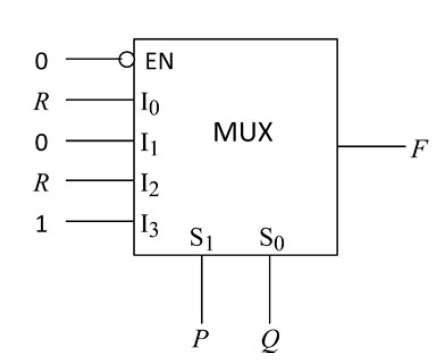
\includegraphics[width=0.5\columnwidth]{figs/2020-gate-ec-10.png}
\caption{}
\label{fig:2020/gate/ec/10}
\end{figure}
%
\item
	The four variable function $f$ is given in terms of min-terms as
\hfill (GATE EC 1991)
		\begin{align*}
	    f(A,B,C,D) = \sum m(2,3,8,10,11,12,14,15)
%\label{eq:1991/gate/ec/9}
		\end{align*}
	    Using the K-map minimize the function in the sum of products form. 
\label{prob:1991/gate/ec/9}
\item Find the logic realized by the circuit in  
\figref{fig:1992/gate/ec/1/22}.
\hfill (GATE EC 1992)
\label{prob:1992/gate/ec/1/22}
\begin{figure}[H]
\centering
	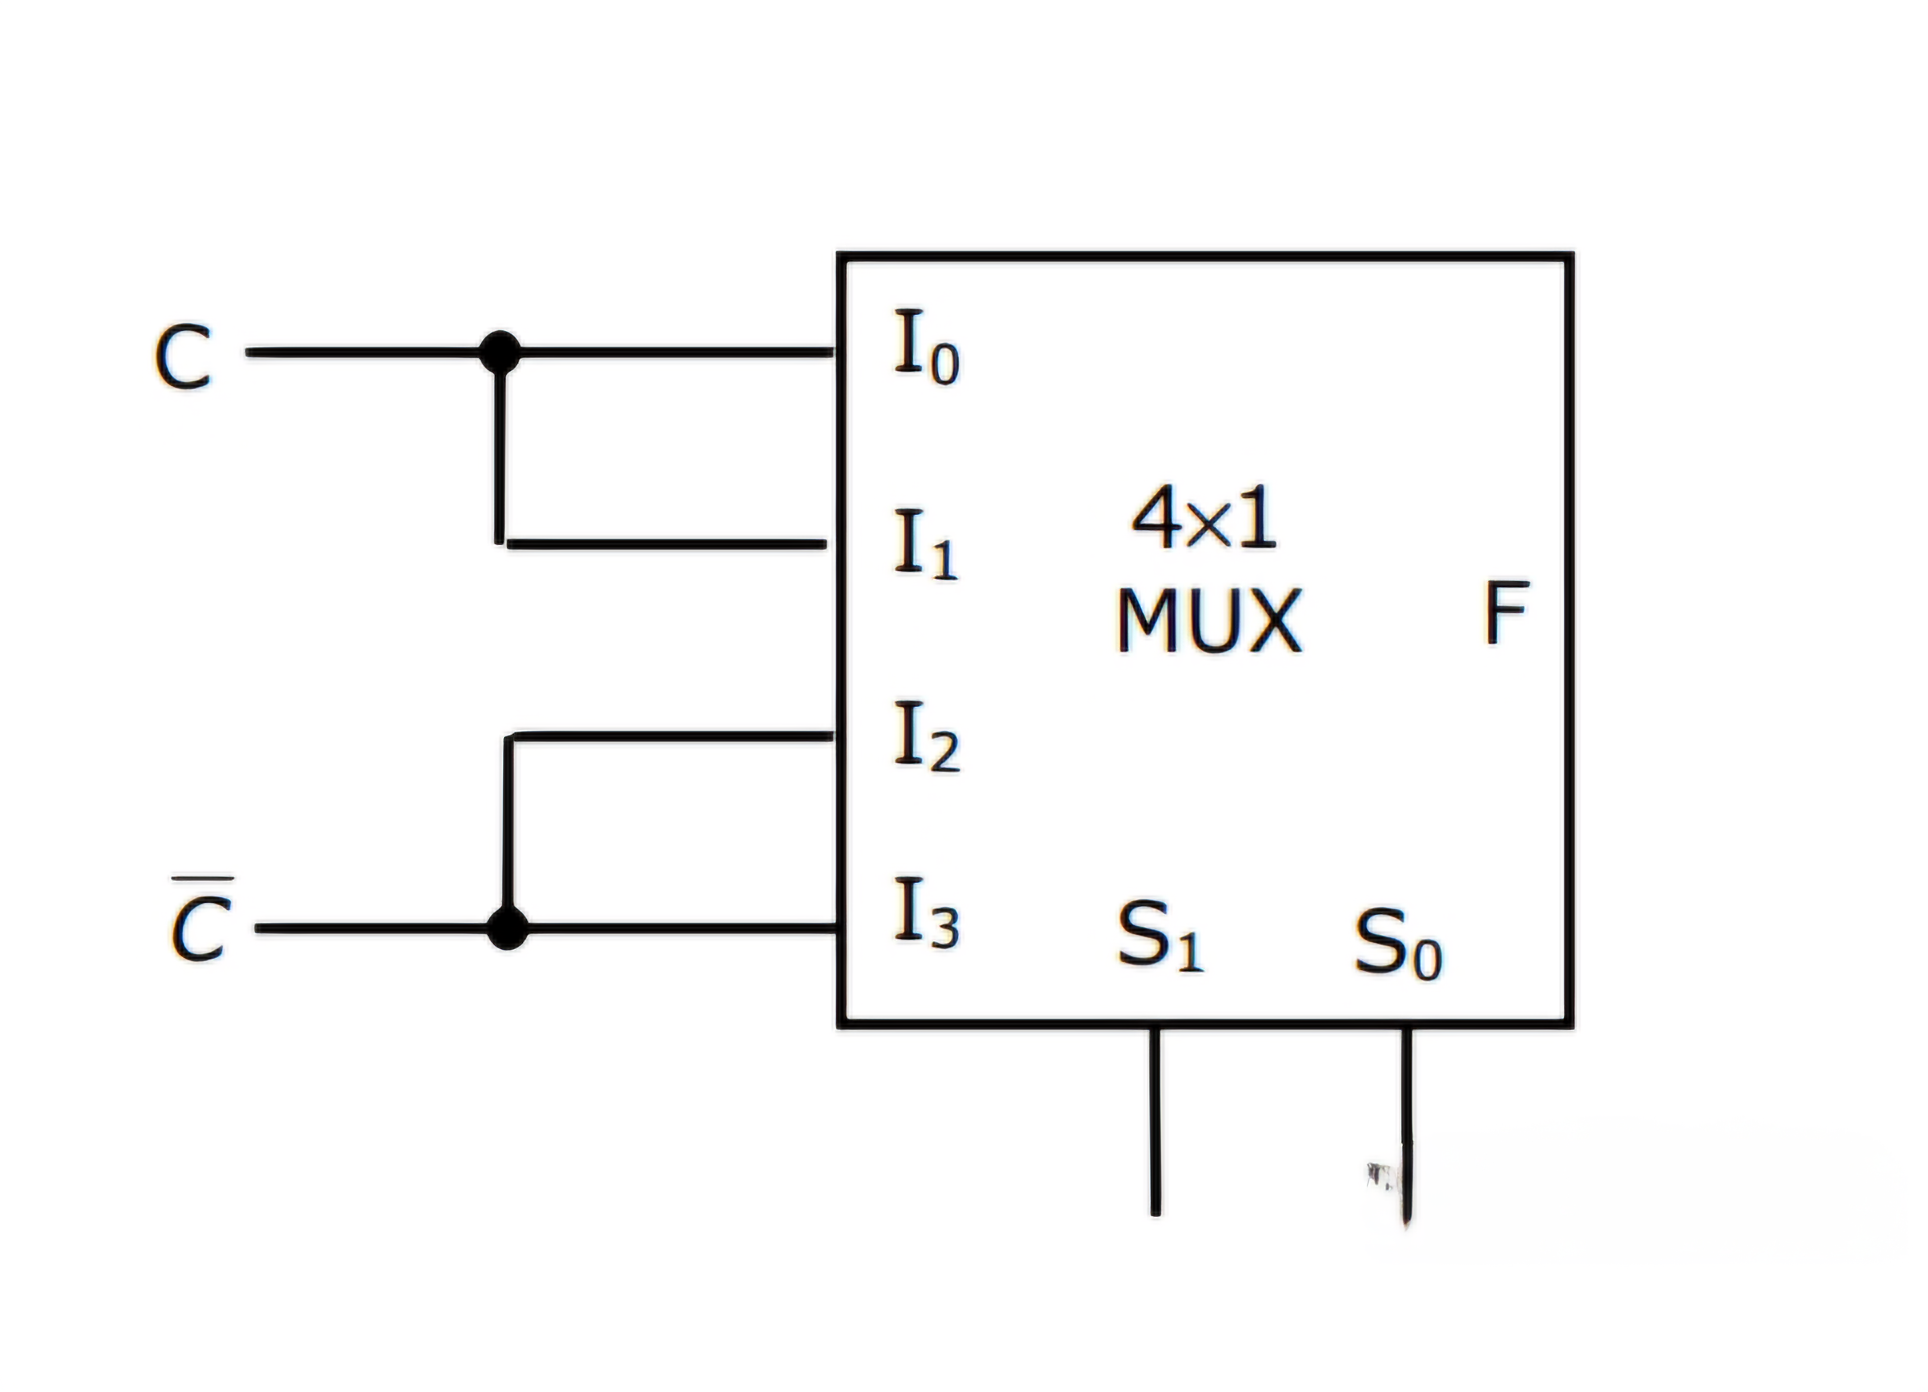
\includegraphics[width=0.5\columnwidth]{figs/1992-gate-ec-1-22.png}
\caption{}
\label{fig:1992/gate/ec/1/22}
\end{figure}
\item
	A combinational circuit has three inputs A, B and C and an output F. F is true only for the following input combinations. 
\hfill (GATE EC 1992)
\label{prob:1992/gate/ec/2/9}
	\begin{enumerate}
		\item A is false and B is true 
		\item A is false and C is true 
		\item A, B and C are all false 
		\item A, B and C are all true 
	\end{enumerate}
	Now, do the following.
	\begin{enumerate}
\item Write the truth table for F. use the convention, true = 1 and false = 0. 
\item Write the simplified expression for F as a sum of products. 
\item Write the simplified expression for F as a product of Sums.
\end{enumerate}
\item Draw the logic circuit for Table 
\ref{tab:1993/gate/ec/5/7} using only NOR gates.
\label{prob:1993/gate/ec/5/7}
\hfill (GATE EC 1993)
	\begin{table}[H]
		\centering
		\begin{tabular}{|c|c|c|c|}
\hline
\textbf{C} &\textbf{B} & \textbf{A} & \textbf{Y} \\
\hline
0 & 0 & 0 & 1 \\  
\hline
0 & 0 & 1 & 1 \\ 
\hline
0 & 1 & 0 & 1 \\
\hline
0 & 1 & 1 & 0 \\
\hline
1 & 0 & 0 & 1 \\  
\hline
1 & 0 & 1 & 0 \\ 
\hline
1 & 1 & 0 & 0 \\
\hline
1 & 1 & 1& 0\\
\hline
\end{tabular}
\caption{}
\label{tab:1993/gate/ec/5/7}
\end{table}
\item
	Implement the following Boolean function in a $8\times1$ multiplexer.
\label{prob:1993/gate/ec/14}
\hfill (GATE EC 1993)
		\begin{align*}
%\label{eq:1993/gate/ec/14}
 Q = BC + ABD' + A'C'D  
		\end{align*}
	\item Minimize the following Boolean function. 
\label{prob:1999/gate/ec/2/10}
		\begin{equation}
F= A'B'C'+A'BC'+A'BC+ABC'
\end{equation}
%
\item Find the Boolean expression for 
\tabref{tab:2005-gate-ec-54}.
\label{prob:2005-gate-ec-54}
\hfill (GATE EC 2005)
	\begin{table}[H]
		\centering
    \begin{tabular}{|l|c|c|c|c|c|c|c|c} \hline \textbf{A}
  & \textbf{B} & \textbf{C} & \textbf{X} \\
 \hline
        0&0&0&0 \\
        \hline
        0&0&1&0 \\
        \hline
        0&1&0&0 \\
        \hline
        0&1&1&1 \\
        \hline
        1&0&0&0 \\
        \hline
        1&0&1&0 \\
        \hline
        1&1&0&1 \\
        \hline
        1&1&1&0  \\
        \hline
\end{tabular}   
\caption{}
\label{tab:2005-gate-ec-54}
\end{table}
\item Minimize the logic function represented by the following Karnaugh map in 
\figref{fig:2021-cbse}.
%\label{prob:2010-gate-ee-52}

\hfill (CBSE 2021)
\begin{figure}[H]
	\centering
\resizebox {0.5\columnwidth} {!} {
	%\begin{karnaugh-map}[4][2][1][$YZ$][$X$]
	\begin{karnaugh-map}[4][2][1][][]
		\manualterms{1,1,0,1,0,0,0,1}
	%	\implicant{0}{1}
	%	\implicant{3}{7}
    \draw[color=black, ultra thin] (0, 2) --
    node [pos=0.7, above right, anchor=south west] {$YZ$} % Y label
    node [pos=0.7, below left, anchor=north east] {$X$} % X label
    ++(135:1);
	\end{karnaugh-map}	
}
\caption{}
\label{fig:2021-cbse}
\end{figure}
\item Find the output for the Karnaugh map shown below
	in
\figref{fig:2019-gate-ee}
%\label{tab:2019-gate-ec-34}
\hfill (GATE EE 2019)
%\begin{figure}[!htb]
\begin{figure}[H]
	\centering
\resizebox {0.5\columnwidth} {!} {
	\begin{karnaugh-map}[4][4][1][][]

		\minterms{1,3,4,5,7,6,12,13,15,14}
		\maxterms{0,2,8,9,10,11}
    \draw[color=black, ultra thin] (0, 4) --
    node [pos=0.7, above right, anchor=south west] {$PQ$} % Y label
    node [pos=0.7, below left, anchor=north east] {$RS$} % X label
    ++(135:1);
%		\implicant{4}{14}
%		\implicant{1}{7}
	\end{karnaugh-map}
}
\caption{}
\label{fig:2019-gate-ee}
\end{figure}
\item 
\label{prob:2021-gate-ec-31}
If all the inputs $P, Q, R, S$ and $T$ are applied simultaneously and held constant in
\figref{fig:2021-gate-ec-31},
find the output $Y$.
\hfill (GATE EC 2021)
\begin{figure}[H]
	\centering
	\resizebox{0.75\columnwidth}{!}{%
\input{gate/2021/31/figs/diagram.tex}
	}
	\caption{}
\label{fig:2021-gate-ec-31}
\end{figure}
\item 
\label{prob:2012-gate-ec-19}
Consider the 2-bit multiplexer (MUX) shown in 
\figref{fig:2012-gate-ec-19}.
	For output to be the XOR of $R$ and $S$, the values for $ W,X,Y$ and $Z$ are \rule{1cm}{0.5pt}.
\hfill (GATE EC 2022)
\begin{enumerate}
\item $W = 0, X = 0, Y = 1, Z = 1$
\item $W = 1, X = 0, Y = 1, Z = 0$
\item $W = 0, X = 1, Y = 1, Z = 0$
\item $W = 1, X = 1, Y = 0, Z = 0$
\end{enumerate}
\begin{figure}[H]
	\centering
	\resizebox{0.4\columnwidth}{!}{%

\begin{circuitikz}

\draw (7,2)coordinate (E) -- (9,2)coordinate (F) -- (9,-1)coordinate (G) -- (7,-1)coordinate (H) -- (7,2)coordinate (E);
\draw (11,2)coordinate (I) -- (13,2)coordinate (J) -- (13,-1)coordinate (K) -- (11,-1)coordinate (L) -- (11,2)coordinate (I);
% AND Gate
\draw (6,1.5) node[and port] (and) {};
\draw (and.in 1) node[left] {};
\draw (and.in 2) node[left] {};
\draw (and.out) |- ($(E)!0.2!(H)$)--++(0:0)node[right]{$D1$}; % and gate output is connected to d1.

%clock
\draw ($(L)!0.5!(K)$)node[anchor=south]{$clk$};
\draw ($(H)!0.5!(G)$)node[anchor=south]{$clk$};
\draw(6,-2) node[above]{$12 \textsl{KHz}$} |- (12,-2);
\draw ($(H)!0.5!(G)$)node[anchor=south,xshift=6]{}--++(90:-1)--++(0:0)node[left]{};
\draw ($(L)!0.5!(K)$)node[anchor=south,xshift=6]{}--++(90:-1)--++(0:0)node[left]{};

\draw($(F)!0.2!(G)$)node[left]{$Q1$} -- ($(I)!0.2!(L)$)node[right]{$D2$}; % q1 is connected to d2.
    
\draw($(F)!0.8!(G)$)node[left]{$\overline{Q1}$};
    
\draw($(J)!0.2!(K)$)node[left]{$Q2$};
    
\draw($(J)!0.8!(K)$)node[left]{$\overline{Q2}$};
    
    
\draw ($(J)!0.2!(K)$)--++(0:1)node[right]{};
    
\draw(and.in 1) --++(90:2)-|(9.5,1)|-($(F)!0.8!(G)$)(0:0)node[left]{}; % and gate input 1 is connected to q1 bar.
    
\draw(and.in 2) --++(-90:4)-|(13.5,-0.5)|- ($(J)!0.8!(K)$);  % and gate input 2 is connected to q2 bar.
    
\end{circuitikz}

	}
\caption{}
\label{fig:2012-gate-ec-19}
\end{figure}
\item $A=a_1a_0$ and $B=b_1b_0$ are two 2-bit unsigned binary numbers. If $F(a_1,a_0,b_1,b_0)$ is a Boolean function such that $F = 1$ only when $A>B$, and $F=0$ otherwise, then $F$ can be minimized to the form \rule{9mm}{0.4pt}.
\hfill(GATE IN 2022)
\label{prob:2022-gate-in-48}
\item
 A $4 \times 1$ multiplexer with two selector lines is used to realize a Boolean function $F$ having four Boolean variables $X$, $Y$, $Z$, and $W$ as shown below in
\figref{fig:4MUX}.
$S_0$ and $S_1$ denote the least significant bit (LSB) and most significant bit (MSB) of the selector lines of the multiplexer, respectively. $I_0$, $I_1$, $I_2$, $I_3$ are the input lines of the multiplexer.
The canonical sum of product representation of $F$ is
\hfill (GATE IN 2021)
\begin{enumerate}
  \item $F(X, Y, Z, W) = \Sigma m(0,1,3,14,15)$
  \item $F(X, Y, Z, W) = \Sigma m(0,1,3,11,14)$
  \item $F(X, Y, Z, W) = \Sigma m(2,5,9,11,14)$
  \item $F(X, Y, Z, W) = \Sigma m(1,3,7,9,15)$
\end{enumerate}
\begin{figure}[H]
	\centering
	\resizebox{0.5\columnwidth}{!}{%
\input{gate/2021/35/figs/multiplexer.tex}
	}
\caption{}
\label{fig:4MUX}
\end{figure}
%
            \item 
            \label{prob:gate IN 35}
            $X = X_1X_0$ and $Y = Y_1Y_0$ are 2-bit binary numbers. The Boolean function $S$ that satisfies the condition ``If $X \textgreater Y$, then $S= 1$", in its minimized form, is 
                  \begin{enumerate}
 
                        \item$X_1Y_1$+$X_0Y_0$
                        \item$X_1\overline{Y_1}+X_0\overline{Y_0}\overline{Y_1}+X_0\overline{Y_0}X_1$
                        \item$X_1\overline{Y_1}X_0\overline{Y_0}$
                        \item$X_1Y_1+X_0\overline{Y_0}Y_1+X_0\overline{Y_0}\overline{X_1}$
                  \end{enumerate}
            \hfill(GATE IN 2019)
%
\item
	\label{prob:2023-gate-ec-9}
	A function $F(A, B, C)$ defined by three Boolean variables A, B and C when expressed as sum of products is given by $$ F = \brak{\overline{A}  \overline{B}  \overline{C}} + \brak{\overline{A}  B  \overline{C}} + \brak{A  \overline{B}  \overline{C}} $$
where, $\overline{A},\overline{B}$ and $\overline{C}$ are the complements of the respective variables. The product of sums (POS) form of the function $F$ is
\hfill(GATE EC 2018)
%
\begin{enumerate}
	\item $ \brak{A+B+C}  \brak{A+\overline{B}+C}  \brak{\overline{A}+B+C} $
 	\item $ \brak{\overline{A}+\overline{B}+\overline{C}}  \brak{\overline{A}+B+\overline{C}}  \brak{A+\overline{B}+\overline{C}} $
	\item $ \brak{A+B+\overline{C}}  \brak{A+\overline{B}+\overline{C}}  \brak{\overline{A}+B+\overline{C}}  \brak{\overline{A}+\overline{B}+C}  \brak{\overline{A}+\overline{B}+C} $
	\item $ \brak{\overline{A}+\overline{B}+C}  \brak{\overline{A}+B+C}  \brak{A+\overline{B}+C}  \brak{A+B+\overline{C}}  \brak{A+B+C} $
\end{enumerate}
\item
\label{prob:gate IN 43}
The product of sun expression of a Boolean function
                is given by 
                \begin{align}
			F(A,B,C)=(A+B+\overline{C})(A+\overline{B}+\overline{C})
			(\overline{A}+B+C)(\overline{A}+\overline{B}+\overline{C})
                \end{align}
                The canonical sum of product expression of $F(A,B,C)$ is given by 
		\hfill(GATE IN 2018)
                 \begin{enumerate}
 
            \item$\overline{A}\overline{B}C+\overline{A}BC+A\overline{B}\overline{C}+ABC$
            \item$\overline{ABC}+\overline{A}B\overline{C}+A\overline{B}C+AB\overline{C}$
            \item$A B\overline{C}+A\overline{B C}+\overline{A}B C+\overline{ABC}$
            \item$\overline{ABC}+\overline{A}BC+AB\overline{C}+ABC$
                  \end{enumerate}
\item
	\label{prob:gate EC 31}
	A four-variable Boolean function is realized using $4\times 1$ multiplexers as shown in the 
        \figref{fig:mux}.
   The minimized expression for $F$ is
    \hfill(GATE EC 2018)
    \begin{enumerate}
       \item $\left ( UV+\bar{U}\bar{V} \right )\bar{W}$
       \item $\left ( UV+\bar{U}\bar{V} \right )\left ( \bar{W}\bar{X}+\bar{W}X\right )$
       \item $\left ( U\bar{V}+\bar{U}V \right )\bar{W}$
       \item $\left ( U\bar{V}+\bar{U}V \right )\left ( \bar{W}\bar{X}+\bar{W}X\right )$
    \end{enumerate}
    \begin{figure}[H]
        \centering
        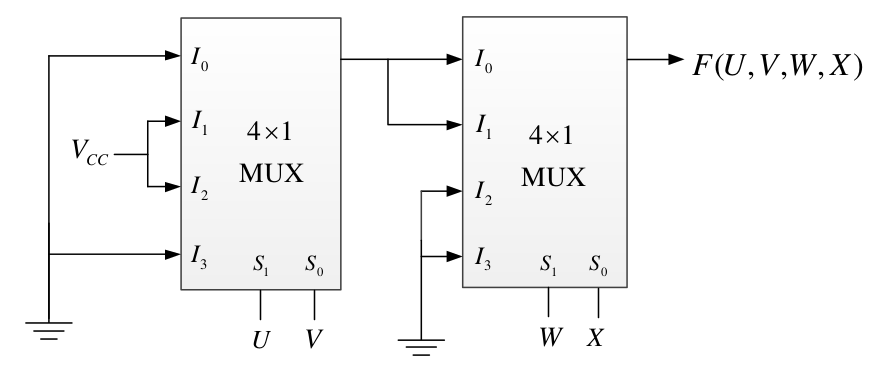
\includegraphics[width=0.75\columnwidth]{figs/2018-gate-ec-31.png}
        \caption{}
        \label{fig:mux}
    \end{figure}
    \item 
  \label{prob:gate  CS-5}
In the Karnaugh map shown below in \figref{fig:GATE EC 2008}, X denotes a don't care term. What is the minimal form of the function represented by the Karnaugh map?
\begin{enumerate}
  \item $ b'd'+a'd' $
  \item $ a'b'+b'd'+a'bd' $
  \item $ b'd'+a'bd' $
  \item $ a'b'+b'd'+a'd' $
\end{enumerate}
\hfill(GATE EC 2008)
    \begin{figure}[H]
\centering
\resizebox{0.5\columnwidth}{!}{%
\begin{karnaugh-map}[4][4][1][][]
    \maxterms{3,5,6,7,11,13,14,15}
    \minterms{0,1,2,8,9}
    \terms{4,10,12}{X} 
    % note: posistion for start of \draw is (0, Y) where Y is
    % the Y size(number of cells high) in this case Y=2
    \draw[color=black, ultra thin] (0, 4) --
    node [pos=0.7, above right, anchor=south west] {$ba$} % Y label
    node [pos=0.7, below left, anchor=north east] {$cd$} % X label
    ++(135:1);
   \end{karnaugh-map}
	    }
        \caption{}
        \label{fig:GATE EC 2008}
    \end{figure}
\iffalse
    \item 
        \label{prob:gate EC 9}
	 In the circuit shown below in \figref{fig:GATE EC 2018}, assume that the comparators are ideal and all components have zero propagation delay . In one period of the input signal Vin=6sin(wt),the fraction of the time which the output OUT is in login state HIGH is 

\begin{figure}[H]
	\centering
	\resizebox{0.75\columnwidth}{!}{%
\begin{tikzpicture}
\tikzset{every picture/.style={line width=0.75pt}} %set default line width to 0.75pt        
%Straight Lines [id:da497014729381388] 
\draw    (140,132.6) -- (169,132.6) ;
%Flowchart: Extract [id:dp3321780746660581] 
\draw   (219,116) -- (169,151) -- (169,81) -- cycle ;
%Straight Lines [id:da17793857448296313] 
\draw    (38,99) -- (166,98) ;
%Straight Lines [id:da9757576729769633] 
\draw    (38,99) -- (39,182) ;
%Straight Lines [id:da772216831020951] 
\draw    (64,100) -- (64,241) ;
%Straight Lines [id:da17160688891184805] 
\draw    (140,132.6) -- (141,160) ;
%Flowchart: Extract [id:dp1753151070852037] 
\draw   (218,262.1) -- (177.82,296.89) -- (178.18,226.9) -- cycle ;
%Straight Lines [id:da8490718483620778] 
\draw    (64,241) -- (178,242) ;
%Straight Lines [id:da2131290241855488] 
\draw    (147,278) -- (146,304) ;
%Straight Lines [id:da06754998827437309] 
\draw    (147,278) -- (178,279) ;
%Straight Lines [id:da6585658480786443] 
\draw    (128,159.5) -- (154,160.5) ;
%Straight Lines [id:da38485782506888055] 
\draw    (131.5,304) -- (139.2,304) -- (160.5,304) ;
%Straight Lines [id:da9940160044670818] 
\draw    (219,116) -- (309,120) ;
%Shape: Not/Inverter Gate [id:dp6645899938254611] 
\draw   (323.81,90) -- (368.26,120) -- (323.81,150) -- (323.81,90) -- cycle (309,120) -- (323.81,120) (377.15,120) -- (389,120) (368.26,120) .. controls (368.26,116.69) and (370.25,114) .. (372.7,114) .. controls (375.16,114) and (377.15,116.69) .. (377.15,120) .. controls (377.15,123.31) and (375.16,126) .. (372.7,126) .. controls (370.25,126) and (368.26,123.31) .. (368.26,120) -- cycle ;
%Shape: Not/Inverter Gate [id:dp5203526386809565] 
\draw   (321.81,169) -- (366.26,199) -- (321.81,229) -- (321.81,169) -- cycle (307,199) -- (321.81,199) (375.15,199) -- (387,199) (366.26,199) .. controls (366.26,195.69) and (368.25,193) .. (370.7,193) .. controls (373.16,193) and (375.15,195.69) .. (375.15,199) .. controls (375.15,202.31) and (373.16,205) .. (370.7,205) .. controls (368.25,205) and (366.26,202.31) .. (366.26,199) -- cycle ;
%Shape: And Gate [id:dp9113043452641065] 
\draw   (453,129) -- (477,129) .. controls (490.25,129) and (501,142.44) .. (501,159) .. controls (501,175.56) and (490.25,189) .. (477,189) -- (453,189) -- (453,129) -- cycle (437,139) -- (453,139) (437,179) -- (453,179) (501,159) -- (517,159) ;
%Straight Lines [id:da5047558236731997] 
\draw    (389,120) -- (438,120) ;
%Straight Lines [id:da7853309017572672] 
\draw    (438,120) -- (437,139) ;
%Straight Lines [id:da09581339031746183] 
\draw    (437,179) -- (438,201) ;
%Straight Lines [id:da16150015131708795] 
\draw    (233.2,117.3) -- (234,256) ;
%Straight Lines [id:da3982360427353082] 
\draw    (218,262.1) -- (402,265) ;
%Straight Lines [id:da7763866390601679] 
\draw    (307.2,221.3) -- (310,263.55) ;
%Shape: And Gate [id:dp6929958094484654] 
\draw   (442,247) -- (466,247) .. controls (479.25,247) and (490,260.44) .. (490,277) .. controls (490,293.56) and (479.25,307) .. (466,307) -- (442,307) -- (442,247) -- cycle (426,257) -- (442,257) (426,297) -- (442,297) (490,277) -- (506,277) ;
%Straight Lines [id:da5339653129723407] 
\draw    (234,256) -- (426,257) ;
%Straight Lines [id:da3839391248130781] 
\draw    (307,199) -- (307.2,221.3) ;
%Straight Lines [id:da6726109915230507] 
\draw    (387,199) -- (438,201) ;
%Straight Lines [id:da40951430114554754] 
\draw    (402,265) -- (403.2,298.3) ;
%Straight Lines [id:da9775921532117686] 
\draw    (403.2,298.3) -- (426,297) ;
%Flowchart: Connector [id:dp8541564806415127] 
\draw   (27.9,195.15) .. controls (27.9,187.89) and (32.87,182) .. (39,182) .. controls (45.13,182) and (50.1,187.89) .. (50.1,195.15) .. controls (50.1,202.41) and (45.13,208.3) .. (39,208.3) .. controls (32.87,208.3) and (27.9,202.41) .. (27.9,195.15) -- cycle ;
%Shape: Sine Wave Form [id:dp42157572682524824] 
\draw   (33,195.15) .. controls (35.44,203.92) and (36.59,203.96) .. (39,195.15) .. controls (41.41,186.34) and (42.54,186.28) .. (45,195.15) ;
%Shape: Or Gate [id:dp7839680372805569] 
\draw   (592,191) -- (612,191) .. controls (625.95,191.54) and (638.42,203.23) .. (644,221) .. controls (638.42,238.77) and (625.95,250.46) .. (612,251) -- (592,251) .. controls (600.57,232.44) and (600.57,209.56) .. (592,191) -- cycle (580,201) -- (596,201) (580,241) -- (596,241) (644,221) -- (660,221) ;
%Straight Lines [id:da1579523714650295] 
\draw    (517,159) -- (580.2,159.3) ;
%Straight Lines [id:da6248594806976522] 
\draw    (506,277) -- (582.2,280.3) ;
%Straight Lines [id:da07782234715989711] 
\draw    (580.2,159.3) -- (580,201) ;
%Straight Lines [id:da20731054042333286] 
\draw    (580,241) -- (582.2,280.3) ;
%Straight Lines [id:da4591115076560359] 
\draw    (193.2,70.3) -- (193.2,98.3) ;
%Straight Lines [id:da9614915073120633] 
\draw    (191,136) -- (191.2,160.3) ;
%Straight Lines [id:da6267154334794827] 
\draw    (200,279) -- (201.2,303.3) ;
%Straight Lines [id:da7013095252421617] 
\draw    (200,222) -- (201.2,247.3) ;
%Straight Lines [id:da505762670676958] 
\draw    (141.2,316.3) -- (151.2,316.3) ;
%Straight Lines [id:da5523950339641612] 
\draw    (175,98) -- (186.2,99.3) ;
%Straight Lines [id:da3727188903283414] 
\draw    (138.2,310.3) -- (154.2,310.3) ;
\draw   (174,129.65) -- (183.2,129.65)(178.6,125) -- (178.6,134.3) ;
\draw   (180,278.3) -- (193.2,278.3)(186.6,273.3) -- (186.6,283.3) ;
%Straight Lines [id:da6667775045429274] 
\draw    (180,247) -- (192.2,247.3) ;
%Shape: Circle [id:dp7754800448867729] 
\draw   (660,221) .. controls (660,219.04) and (661.59,217.45) .. (663.55,217.45) .. controls (665.51,217.45) and (667.1,219.04) .. (667.1,221) .. controls (667.1,222.96) and (665.51,224.55) .. (663.55,224.55) .. controls (661.59,224.55) and (660,222.96) .. (660,221) -- cycle ;
%Straight Lines [id:da3040090400300808] 
\draw    (39,208.3) -- (39.2,239.6) ;
%Straight Lines [id:da6746368970911716] 
\draw    (23.2,241.3) -- (55.2,240.3) ;
%Straight Lines [id:da7013568848674232] 
\draw    (32,249) -- (47.2,248.3) ;
%Straight Lines [id:da40668201779662905] 
\draw    (36,256) -- (44.2,255.3) ;

% Text Node
\draw (199.7,56.16) node  [rotate=-359.96] [align=left] {\begin{minipage}[lt]{27.88pt}\setlength\topsep{0pt}
HIGH
\end{minipage}};
% Text Node
\draw (190.6,170.15) node   [align=left] {\begin{minipage}[lt]{28.02pt}\setlength\topsep{0pt}
LOW
\end{minipage}};
% Text Node
\draw (201.78,207.75) node   [align=left] {\begin{minipage}[lt]{32.1pt}\setlength\topsep{0pt}
HIGH
\end{minipage}};
% Text Node
\draw (200.1,314.75) node   [align=left] {\begin{minipage}[lt]{28.7pt}\setlength\topsep{0pt}
LOW
\end{minipage}};
% Text Node
\draw (669.1,198.75) node   [align=left] {\begin{minipage}[lt]{25.98pt}\setlength\topsep{0pt}
OUT
\end{minipage}};
% Text Node
\draw (12.13,170) node  [rotate=-358.82] [align=left] {\begin{minipage}[lt]{23.22pt}\setlength\topsep{0pt}
6sin(wt)
\end{minipage}};
% Text Node
\draw (146.6,170.65) node   [align=left] {\begin{minipage}[lt]{25.3pt}\setlength\topsep{0pt}
3 V
\end{minipage}};
\end{tikzpicture}
}
        \caption{}
        \label{fig:GATE EC 2018}
    \end{figure}

\begin{enumerate}
    \item $\frac{1}{12}$
    \item $\frac{1}{2}$
    \item $\frac{2}{3}$
    \item $\frac{5}{6}$
\end{enumerate}
\hfill(GATE EC 2018)




  \item 
  \label{prob:gate  IN 46}
  The Boolean function $F\brak{X,Y}$ realized by the given circuit 
  in \figref{fig:GATE IN 2019} is
  
  \begin{figure}[H]
	  \centering
	  \resizebox{0.5\columnwidth}{!}{%
\begin{tikzpicture}
%\begin{tikzpicture}[x=0.75pt,y=0.75pt,yscale=-1,xscale=1]
% Your original TikZ code here
%\tikzset{every picture/.style={line width=0.75pt}} %set default line width to 0.75pt        

%Straight Lines [id:da8870235423908663] 
\draw    (99.2,109.6) -- (136.21,109.78) -- (173.2,109.6) ;
%Flowchart: Delay [id:dp3076178503272544] 
\draw   (174,96) -- (209,96) .. controls (228.33,96) and (244,111.67) .. (244,131) .. controls (244,150.33) and (228.33,166) .. (209,166) -- (174,166) -- cycle ;
%Straight Lines [id:da4880418888531195] 
\draw    (99.2,149.6) -- (111.2,149.6) -- (166.2,149.6) -- (174.2,149.6) ;
%Shape: Circle [id:dp4693486828792446] 
\draw   (244,131) .. controls (244,128.18) and (246.28,125.9) .. (249.1,125.9) .. controls (251.92,125.9) and (254.2,128.18) .. (254.2,131) .. controls (254.2,133.82) and (251.92,136.1) .. (249.1,136.1) .. controls (246.28,136.1) and (244,133.82) .. (244,131) -- cycle ;
%Straight Lines [id:da4653941185722381] 
\draw    (254.2,131) -- (288.2,130.6) ;
%Straight Lines [id:da8761511817778416] 
\draw    (39.2,30.6) -- (329.2,29.6) ;
%Straight Lines [id:da1606414736134072] 
\draw    (42.2,239.6) -- (332.2,238.6) ;
%Straight Lines [id:da6304107801712311] 
\draw    (288.2,130.6) -- (289.2,70.6) ;
%Straight Lines [id:da9368244337166334] 
\draw    (289.2,70.6) -- (329.2,69.6) ;
%Straight Lines [id:da8466357262704003] 
\draw    (288.2,191.6) -- (288.2,130.6) ;
%Straight Lines [id:da46784195426353525] 
\draw    (288.2,191.6) -- (330.2,191.6) ;
%Flowchart: Delay [id:dp9030516796824679] 
\draw   (330,12) -- (365,12) .. controls (384.33,12) and (400,27.67) .. (400,47) .. controls (400,66.33) and (384.33,82) .. (365,82) -- (330,82) -- cycle ;
%Flowchart: Delay [id:dp09252224992976132] 
\draw   (332,177) -- (367,177) .. controls (386.33,177) and (402,192.67) .. (402,212) .. controls (402,231.33) and (386.33,247) .. (367,247) -- (332,247) -- cycle ;
%Shape: Circle [id:dp5499693136350294] 
\draw   (402,212) .. controls (402,209.18) and (404.28,206.9) .. (407.1,206.9) .. controls (409.92,206.9) and (412.2,209.18) .. (412.2,212) .. controls (412.2,214.82) and (409.92,217.1) .. (407.1,217.1) .. controls (404.28,217.1) and (402,214.82) .. (402,212) -- cycle ;
%Shape: Circle [id:dp74153314191801] 
\draw   (400,47) .. controls (400,44.18) and (402.28,41.9) .. (405.1,41.9) .. controls (407.92,41.9) and (410.2,44.18) .. (410.2,47) .. controls (410.2,49.82) and (407.92,52.1) .. (405.1,52.1) .. controls (402.28,52.1) and (400,49.82) .. (400,47) -- cycle ;
%Straight Lines [id:da35345529297391987] 
\draw    (410.2,47) -- (460.2,46.6) ;
%Straight Lines [id:da8140464066015929] 
\draw    (412.2,212) -- (462.2,211.6) ;
%Flowchart: Delay [id:dp21989758956535077] 
\draw   (502,91) -- (537,91) .. controls (556.33,91) and (572,106.67) .. (572,126) .. controls (572,145.33) and (556.33,161) .. (537,161) -- (502,161) -- cycle ;
%Straight Lines [id:da14664335527509076] 
\draw    (460.2,46.6) -- (461.2,111.6) ;
%Straight Lines [id:da5388257463322341] 
\draw    (461.2,146.6) -- (462.2,211.6) ;
%Straight Lines [id:da4857250526271579] 
\draw    (461.2,111.6) -- (502.2,111.6) ;
%Straight Lines [id:da5555292815908546] 
\draw    (461.2,146.6) -- (502.2,146.6) ;
%Shape: Circle [id:dp793166461459196] 
\draw   (572,126) .. controls (572,123.18) and (574.28,120.9) .. (577.1,120.9) .. controls (579.92,120.9) and (582.2,123.18) .. (582.2,126) .. controls (582.2,128.82) and (579.92,131.1) .. (577.1,131.1) .. controls (574.28,131.1) and (572,128.82) .. (572,126) -- cycle ;
%Straight Lines [id:da6138015275286377] 
\draw    (582.2,126) -- (603.2,125.6) ;
%Straight Lines [id:da6694995059558879] 
\draw    (99.2,109.6) -- (100.2,31.6) ;
%Straight Lines [id:da9757039240740732] 
\draw    (100.2,239.6) -- (99.2,149.6) ;

% Text Node
\draw (22,22) node [anchor=north west][inner sep=0.75pt]   [align=left] {X};
% Text Node
\draw (24,232) node [anchor=north west][inner sep=0.75pt]   [align=left] {Y};
% Text Node
\draw (606,117) node [anchor=north west][inner sep=0.75pt]   [align=left] {F};

  
\end{tikzpicture}
}
\caption{}
\label{fig:GATE IN 2019}
  \end{figure}
\begin{enumerate}
      \item \(\bar{X}Y + X\bar{Y}\)
      \item \(\bar{X}\bar{Y} + XY\)
      \item \(X+Y\)
      \item \(\bar{X}.\bar{Y}\)

      \end{enumerate}
\hfill(GATE IN 2019)
\fi
  \item 
  \label{prob:gate  CS 49 }
 Consider the minterm list form of a Boolean function given below.$$F(P, Q, R, S) = \sum m(0, 2, 5, 7, 9, 11) + d(3, 8, 10, 12, 14)$$
 Here, $m$ denotes a minterm and $d$ denotes a don’t care term. The number of essential prime implicants of the function is \rule{1cm}{0.1pt}.
\hfill (GATE CS 2018)
%
 \item The simplified form of the Boolean function $F(W,X,Y,Z)=\sum(4,5,10,11,12,13,14,15)$ with the minimum number of terms and smallest number of literals in each terms is \rule{1cm}{0.1pt}.
 \hfill{(GATE IN 2023)}
	  \begin{enumerate}
		  \item $WX+\bar WX\bar Y+W\bar XY$
		   \item $WX+WY+X\bar Y$
		     \item $X\bar Y+WY$
		      \item$\bar XY+\bar W\bar Y$
	\end{enumerate}
%
\item Q, R, S are Boolean variables  $ \oplus$ and is the XOR operator. Select the CORRECT option(s).
\hfill{(Gate BM 2023)}
\begin{enumerate}
\item $(Q  \oplus  R)  \oplus  S = Q  \oplus  (R  \oplus  S) $
\item $(Q  \oplus  R)  \oplus  S = 0$ when any of the Boolean variables (Q, R, S) are 0 and the third variable is 1
\item $(Q  \oplus  R)  \oplus  S = 1$ when Q = R = S = 1
\item $((Q  \oplus  R)  \oplus  (R  \oplus  S))  \oplus  (Q  \oplus  S) = 1$
\end{enumerate}
%
\item The output F of the digital circuit shown 
	in \figref{fig:GATE IN 2022}
	can be written in the form(s) \rule{1cm}{0.1pt}.
    \begin{figure}[H]
        \centering
        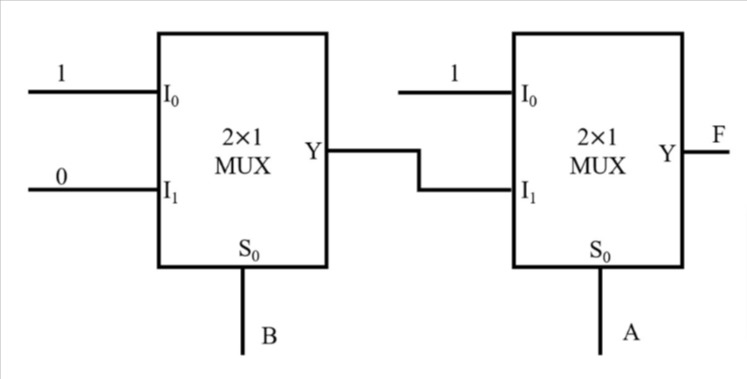
\includegraphics[width=0.75\columnwidth]{figs/gate_in_2022_q23.jpg}
        \caption{}
\label{fig:GATE IN 2022}
    \end{figure}
    \begin{enumerate}
        \item $\overline{A.B}$
        \item $\bar{A}$+$\bar{B}$
        \item $\overline{A + B}$
        \item $\bar{A}$.$\bar{B}$
    \end{enumerate}
    \hfill (GATE IN 2022)

\item $\vec{A}=a_1a_0$ and $\vec{B}=b_1b_0$ are two 2-bit unsigned binary numbers. If $\vec{F}\brak{a_1,a_0,b_1,b_0}$ is a Boolean function such that $\vec{F} = 1$ only when $\vec{A > B}$, and $\vec{F} = 0$ otherwise, then $\vec{F}$ can be minimized to the form $\rule{2.5cm}{0.10mm}$
\begin{enumerate}
\item $a_1\bar{b_1}+a_1a_0\bar{b_0}$
\item $a_1\bar{b_1}+a_1a_0\bar{b_0}+a_0\bar{b_0}\bar{b_1}$
\item $a_1a_0\bar{b_0}+a_0\bar{b_0}\bar{b_1}$
\item $a_1\bar{b_1}+a_1a_0\bar{b_0}+a_0\bar{b_0}b_1$
\end{enumerate}
\hfill(GATE IN 2022)
%
\item In the circuit shown below in 
\figref{fig:fig-1.png},
 $Y$ is a $2$-bit $(Y_1Y_o)$ output of the combinational logic. What is the 
maximum value of $Y$ for any given digital inputs, $A_1A_0$ and $B_1B_0$ ?
\hfill(GATE BM 2021)
\begin{figure}[H]
\centering
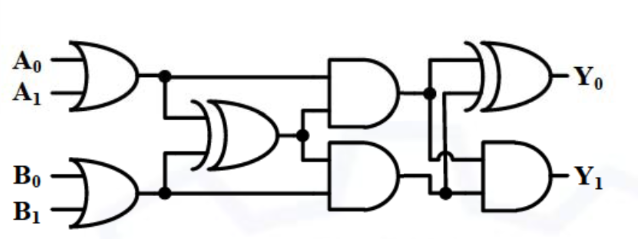
\includegraphics[width=0.5\columnwidth]{ide/kmap/figs/Fig-1.png}
\caption{}
\label{fig:fig-1.png}
\end{figure}
\begin{enumerate}[label=(\Alph*)]
\item $01$
\item $10$
\item $00$
\item $11$
\end{enumerate}
\item Match the Boolean expression with its minimal realization
	in 
		\tabref{fig:GATE BM 2020}
	\begin{table}[H]
		\centering
		\resizebox{0.75\columnwidth}{!}{%
		\begin{tabular}{|c|c|c|c|}
\hline

   & Boolean expression &   &  Minimal realization \\
	\hline 

	$P$ & $\bar{X}\bar{Y}\bar{Z}$ + $\bar{X}Y\bar{Z}$ + $\bar{X}YZ$ & $K$ &  $X(Y+Z)$ \\

	\hline 

	$Q$ & $XYZ$ + $X\bar{Y}Z$ +$XY\bar{Z}$ & $L$ & $\bar{X}(Y+\bar{Z})$ \\

	\hline 

	$R$ & $XY + XYZ +XY\bar{Z} + \bar{X}YZ$ & $M$ & $Z$ \\

	\hline

	$S$ & $\bar{X}\bar{Y}Z + \bar{X}YZ + X\bar{Y}Z$ + $XYZ$ & $N$ & $Y(X+Z)$ \\

	\hline 
\end{tabular}
		}
		\caption{}
		\label{fig:GATE BM 2020}
	\end{table}
		\hfill(GATE BM 2020)
	\begin{enumerate}[label=(\Alph*)]
			\item $P-K$, $Q-L$ ,$R-N$ , $S-M$ \\
			\item $P-L$, $Q-K$, $R-N$, $S-M$ \\
			\item $P-L$ ,$Q-N$, $R-M$, $S-K$ \\
			\item $P-M$, $Q-K$, $R-L$, $S-N$ \\
	\end{enumerate}

\item A $ 4\times1$ multiplexer with two selector lines is used to realize a Boolean function $F$ having four Boolean variables $X, Y, Z$ and $W$ as shown below
in  \figref{fig:multiplexerwithtwoselectionliness}.
	 $S_0$ and $S_1$ denote the least significant bit $\brak{LSB}$ and most significant bit $\brak{MSB}$ of the selector lines of the multiplexer respectively. $I_0, I_1, I_2,I_3$ are the input lines of the multiplexer.

	 \hfill(GATE IN 2021)
  \begin{figure}[H]
  \centering
  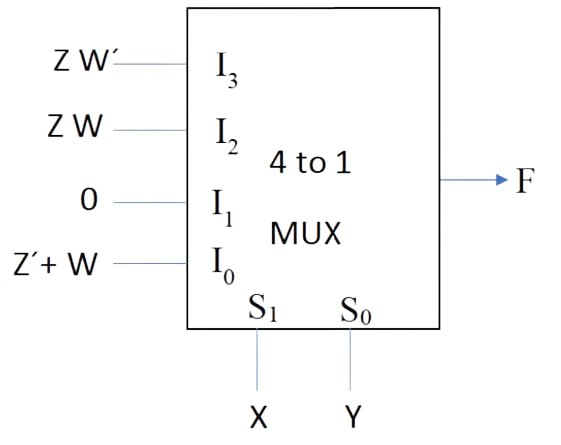
\includegraphics[width=0.4\columnwidth]{figs/kmapsmall.jpg}
  \caption{Multiplexer}
  \label{fig:multiplexerwithtwoselectionliness}
\end{figure}
\textbf{The canonical sum of product representations of $\textbf{F}$ is} 
 \begin{enumerate}
        \item  $F\brak{X,Y,Z,W} = \sum m \brak{0,1,3,14,15}$
        \item  $F\brak{X,Y,Z,W} = \sum m \brak{0,1,3,11,14}$
        \item  $F\brak{X,Y,Z,W} = \sum m \brak{2,5,9,11,14}$
        \item  $F\brak{X,Y,Z,W} = \sum m \brak{1,3,7,9,15}$
    \end{enumerate}
\iffalse
\item The output expression for the Karnaugh map shown below in
                                \figref{fig:GATE-EE2019,35}
				is
                                \hfill(GATE EE 2019)
		\begin{figure}[H]
            \centering		
   		\begin{karnaugh-map}[4][4][1][$PQ$][$RS$]
\minterms{1,3,4,5,6,7,12,13,14,15}
\autoterms[0]
\end{karnaugh-map}

      	\caption{K-MAP}
                                \label{fig:GATE-EE2019,35}
		\end{figure}
\begin{enumerate}
    \item $Q\overline{R} + S$
    \item $Q\overline{R} + \overline{S}$
    \item $QR + S$
    \item $QR + \overline{S}$
\end{enumerate}
\fi
\item The output expression of the Karnaugh map shown below in
\figref{fig:k-map-E}
is

				\hfill(GATE EE 2017)
\begin{figure}[H]
	\centering
\resizebox {0.5\columnwidth} {!} {
	\begin{karnaugh-map}[4][4][1][][]

		\maxterms{0,1,2,3,5,7,8,9,10,11,13}
		\minterms{4,6,12,14,15}
    \draw[color=black, ultra thin] (0, 4) --
    node [pos=0.7, above right, anchor=south west] {$CD$} % Y label
    node [pos=0.7, below left, anchor=north east] {$AB$} % X label
    ++(135:1);
%		\implicant{4}{14}
%		\implicant{1}{7}
	\end{karnaugh-map}
}
\caption{}
\label{fig:k-map-E}
\end{figure}
\iffalse
\begin{figure}[H]
\centering
\begin{circuitikz}
\tikzstyle{every node}=[font=\LARGE]
\draw [](9.25,13.25) to[short] (9.25,9.25);
\draw [](10.25,13.25) to[short] (10.25,9.25);
\draw [](11.25,13.25) to[short] (11.25,9.25);
\draw [](12.25,13.25) to[short] (12.25,9.25);
\draw [](13.25,13.25) to[short] (13.25,9.25);
\draw [](9.25,13.25) to[short] (13.25,13.25);
\draw[] (13.25,9.25) to[short] (9.25,9.25);
\draw [](9.25,12.25) to[short] (13.25,12.25);
\draw [](9.25,11.25) to[short] (13.25,11.25);
\draw [](9.25,10.25) to[short] (13.25,10.25);
\draw [short] (9.25,13.25) -- (7.5,14.75);
\node [font=\LARGE] at (7.75,13.75) {AB};
\node [font=\LARGE] at (8.75,14.25) {CD};
\node [font=\LARGE] at (8.75,12.75) {00};
\node [font=\LARGE] at (8.75,11.75) {01};
\node [font=\LARGE] at (8.75,10.75) {11};
\node [font=\LARGE] at (8.75,9.75) {10};
\node [font=\LARGE] at (9.75,13.5) {00};
\node [font=\LARGE] at (10.75,13.5) {01};
\node [font=\LARGE] at (11.75,13.5) {11};
\node [font=\LARGE] at (12.75,13.5) {10};
\node [font=\LARGE] at (9.75,12.75) {0};
\node [font=\LARGE] at (10.75,12.75) {0};
\node [font=\LARGE] at (11.75,12.75) {0};
\node [font=\LARGE] at (12.75,12.75) {0};
\node [font=\LARGE] at (9.75,11.75) {1};
\node [font=\LARGE] at (9.75,10.75) {1};
\node [font=\LARGE] at (12.75,11.75) {1};
\node [font=\LARGE] at (12.75,10.75) {1};
\node [font=\LARGE] at (11.75,10.75) {1};
\node [font=\LARGE] at (10.75,11.75) {0};
\node [font=\LARGE] at (11.75,11.75) {0};
\node [font=\LARGE] at (10.75,10.75) {0};
\node [font=\LARGE] at (9.75,9.75) {0};
\node [font=\LARGE] at (10.75,9.75) {0};
\node [font=\LARGE] at (11.75,9.75) {0};
\node [font=\LARGE] at (12.75,9.75) {0};
\end{circuitikz}

	\caption{}
\label{fig:k-map-E}
\end{figure}
\fi

\begin{enumerate}
\item $B\overline{D} + BCD$
\item $B\overline{D} + AB$
\item $\overline{B}D + ABC$
\item $B\overline{D} + ABC$
\end{enumerate}

\item A Boolean function $F$ of three variables $X, Y, \text{ and } Z$ is given as 
$F(X, Y, Z) = (X' + Y + Z)(X + Y' + Z') (X' + Y + Z') (X'Y'Z' + X' Y Z' + XYZ')$.

Which one of the following is true?
\hfill(GATE IN 2021)

\begin{enumerate}
    \item $F(X, Y, Z) = (X + Y + Z') (X' + Y' + Z')$
    \item $F(X, Y, Z) = (X'+ Y) (X + Y' + Z')$
    \item $F(X, Y, Z) = X'Z' + YZ'$
    \item $F(X, Y, Z) = X'Y'Z + XYZ$
\end{enumerate}
\item The product of sum expression of a Boolean function $F\brak{A,B,C}$ of three variables is given by
\begin{align*}
F\brak{A,B,C} = \brak{A + B + \bar{C}}\brak{A + \bar{B} +\bar{C}}\brak{\bar{A} + B + C}
\brak{\bar{A} + \bar{B} + \bar{C}}
\end{align*}
The canonical sum of product expression of $F\brak{A,B,C}$ is  given by
  \begin{enumerate}                               
	  \item $\bar{A}\hspace{4pt}\bar{B}\hspace{4pt}C+ \bar{A}\hspace{4pt}B\hspace{4pt}\bar{C} + A\hspace{4pt}\bar{B}\hspace{4pt}C + A\hspace{4pt}B\hspace{4pt}C$
	  \item $\bar{A}\hspace{4pt}\bar{B}\hspace{4pt}\bar{C} + \bar{A}\hspace{4pt}B\hspace{4pt}\bar{C} + A\hspace{4pt}\bar{B} C + A\hspace{4pt}B\hspace{4pt}\bar{C}$
	  \item $A\hspace{4pt}B\hspace{4pt} \bar{C} + A\hspace{4pt}\bar{B}\hspace{4pt}\bar{C} + \bar{A}\hspace{4pt}B\hspace{4pt}C + \bar{A}\hspace{4pt}B\hspace{4pt}C + \bar{A}\hspace{4pt}\bar{B}\hspace{4pt}\bar{C}$
	  \item $\bar{A}\hspace{4pt}\bar{B}\hspace{4pt}\bar{C} + \bar{A}\hspace{4pt}B\hspace{4pt}C +A\hspace{4pt}B\hspace{4pt}\bar{C} + A\hspace{4pt}B\hspace{4pt}\bar{C}+ A\hspace{4pt}B\hspace{4pt}C$
\end{enumerate}
\hfill (GATE IN 2018)
\item Digital input signals $A, B, C$ with $A$ as the MSB and $C$ as the LSB are used to realize the Boolean function $F=m_0+m_2+m_3+m_5+m_7$, where $m_i$ denotes the $i^{th}$ minterm. In addition, $F$ has a don't care for $m_1$. The simplified expression for $F$ is given by 
\begin{enumerate}
    \item $\bar{A} \bar{C}+\bar{B} C+A C$
    \item$\bar{A}+C$
    \item$\bar{C}+A$ 
    \item$\bar{A} C+BC+A\bar{C}$
\end{enumerate}
\hfill (GATE EE 2018)
\item Consider the minterm list form of a Boolean function $F$ given below.
\begin{align*}
	F\brak{P,Q,R,S}=\sum m\brak{0,2,5,7,9,11}+d\brak{3,8,10,12,14}
\end{align*}
Here, $m$ denotes a minterm and $d$ denotes a don't care term.The number of essential prime implicants of the function $F$ is  \rule{1cm}{0.1pt}. 	
	\hfill (GATE CS 2018)
\item Derive a Canonical POS expression for a Boolean function F, represented by 
Table \ref{tab:2019/c/6/c}\hfill (CBSE 2019)
\label{prob:2019/c/6/c}
\begin{table}[H]
\centering
\begin{tabular}{|l|l|l|c|}
	\hline
	X&Y&Z&F(X,Y,Z)\\
	\hline
	0&0&0&1\\
	0&0&1&0\\
	0&1&0&1\\
	0&1&1&0\\
	1&0&0&1\\
	1&0&1&1\\
	1&1&0&0\\
	1&1&1&0\\
	\hline
\end{tabular}
\caption{}
\label{tab:2019/c/6/c}
\end{table}
%
\item 
Find $X$ in the following circuit in 
\figref{fig:2007-gate-ec-43}
\hfill (GATE EC 2007)
\label{prob:2007-gate-ec-43}
\begin{figure}[H]
\centering
	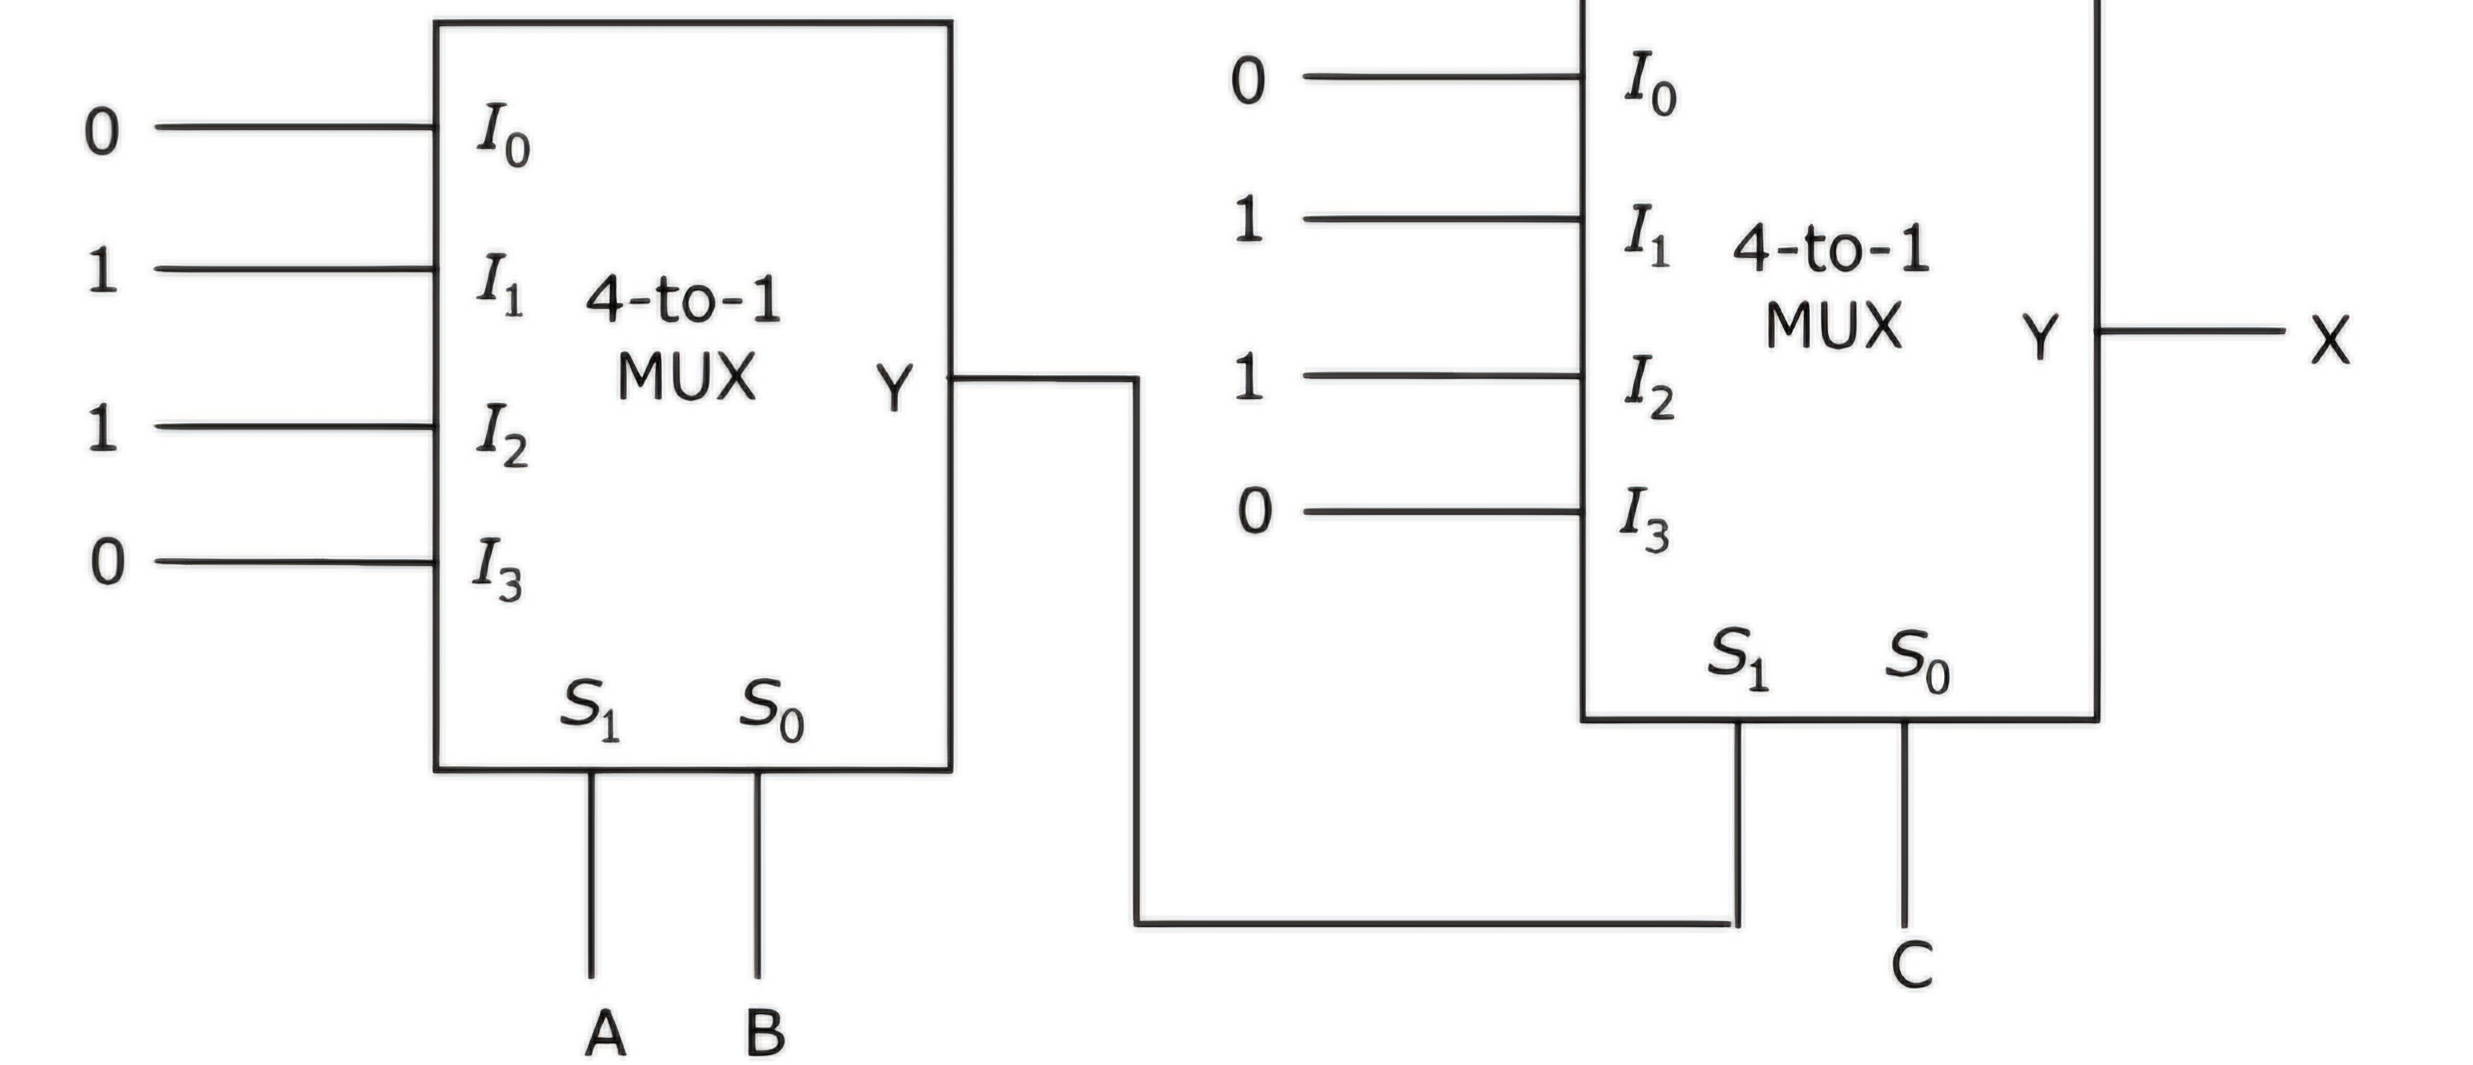
\includegraphics[width=0.75\columnwidth]{figs/2007-gate-ec-43.png}
\caption{}
\label{fig:2007-gate-ec-43}
\end{figure}
\item 
\label{prob:2007-gate-in-10}
      A logic circuit implements the boolean function $F=X'Y+XY'Z'$. It is found that the input combination $X=Y=1$ can never occur. Taking this into account, find a simplified expression for $F$. 
\hfill (GATE IN 2007)
\item 
\label{prob:2010-gate-ec-39}
Find the Boolean logic realised by the following circuit in 
\figref{fig:2010-gate-ec-39}.

\hfill (GATE EC 2010)
\begin{figure}[H]
\centering
	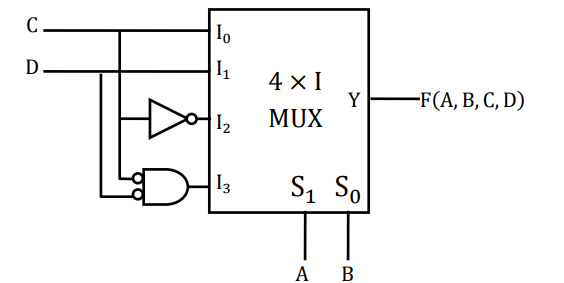
\includegraphics[width=0.5\columnwidth]{figs/2010-gate-ec-39.png}
\caption{}
\label{fig:2010-gate-ec-39}
\end{figure}
\item 
\label{prob:2011-gate-ec-20}
Find the logic function implemented by the circuit given below 
in 
\figref{fig:2011-gate-ec-20}.

\hfill (GATE EC 2011)
\begin{figure}[H]
\centering
	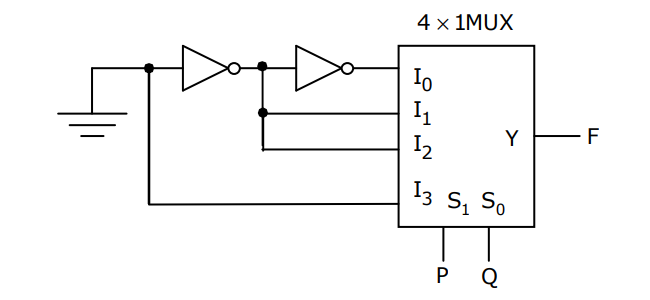
\includegraphics[width=0.75\columnwidth]{figs/2011-gate-ec-20.png}
\caption{}
\label{fig:2011-gate-ec-20}
\end{figure}
    \item The circut shown in  
\figref{fig:block_diagram}
	    comprises of XOR, AND gates and multiplexers.  
    If all the inputs $P, Q, R, S$ and $T$ are applied simultaneously and held constant, find $Y$.

\hfill(GATE EC 2021)  
\begin{figure}[H]
	\centering
	\resizebox{0.75\columnwidth}{!}{
\begin{circuitikz}
\draw (7,1)coordinate (E) -- (8,1)coordinate (F) -- (8,-1)coordinate (G) -- (7,-1)coordinate (H) -- (7,1)coordinate (E);
\draw (11,2)coordinate (I) -- (13,2)coordinate (J) -- (13,-1)coordinate (K) -- (11,-1)coordinate (L) -- (11,2)coordinate (I);
 \draw ($(J)!0.5!(K)$)--++(0:2)node[right]{$Y$};
 \draw ($(L)!0.5!(K)$)node[anchor=south]{$S0$}--++(90:-2)--++(1:-10)node[left]{$T$};
 \draw ($(H)!0.5!(G)$)node[anchor=south]{$S0$}--++(90:-2)--++(1:0)node[left]{};
\draw (4,2) node[and port] (myand1) {};
\draw (myand1.in 1) node (A1)     [anchor=east,xshift=-1cm]           {$P$}
(myand1.in 1) -- (A1);
\draw(4,-2) node[and port] (myand2) {}
(myand2.in 2) node (B2)     [anchor=east,xshift=-1cm]           {$S$};
\draw(myand2.in 2) -- (B2);
\draw (10,0) node[and port] (myand3) {};
\draw (4,0) node[xor port] (myxor) {};
\draw (myand1.in 2) node (B1)     [anchor=east,xshift=-1cm,yshift=-.7cm]  {$Q$};
\draw (B1) -- ++(1.25cm,0);
\draw (myxor.in 1) node (B1)     [anchor=east,xshift=-1cm,yshift=-1.3cm]  {$R$};
\draw (B1) -- ++(1.25cm,0);

\draw (myand1.in 2) |- (myxor.in 1);
\draw (myand2.in 1) |- (myxor.in 2);

\draw (myxor.out) |- ($(E)!0.2!(H)$)--++(0:0)node[right]{$0$};
\draw(myand1.out) |- ($(I)!0.2!(L)$)--++ (0:0)node[right]{$0$};
\draw (myand1.out) -| (myand3.in 1);
\draw(myand3.out) -| ($(I)!0.7!(L)$)--++(0:0)node[right]{$1$};
\draw ($(F)!0.6!(G)$)--++(0:0)node[right]{} -| (myand3.in 2) ;
\draw (myand2.out) |- ($(E)!0.7!(H)$)--++(0:0)node[right]{$1$};

\end{circuitikz}
~


	}
\caption{} 
\label{fig:block_diagram}
\end{figure}
\item 
\label{prob:2017-gate-ec-16}
Find the logic function implemented by the circuit given below 
in 
\figref{fig:2017-gate-ec-16}.

\hfill (GATE EC 2017)
\begin{figure}[H]
\centering
	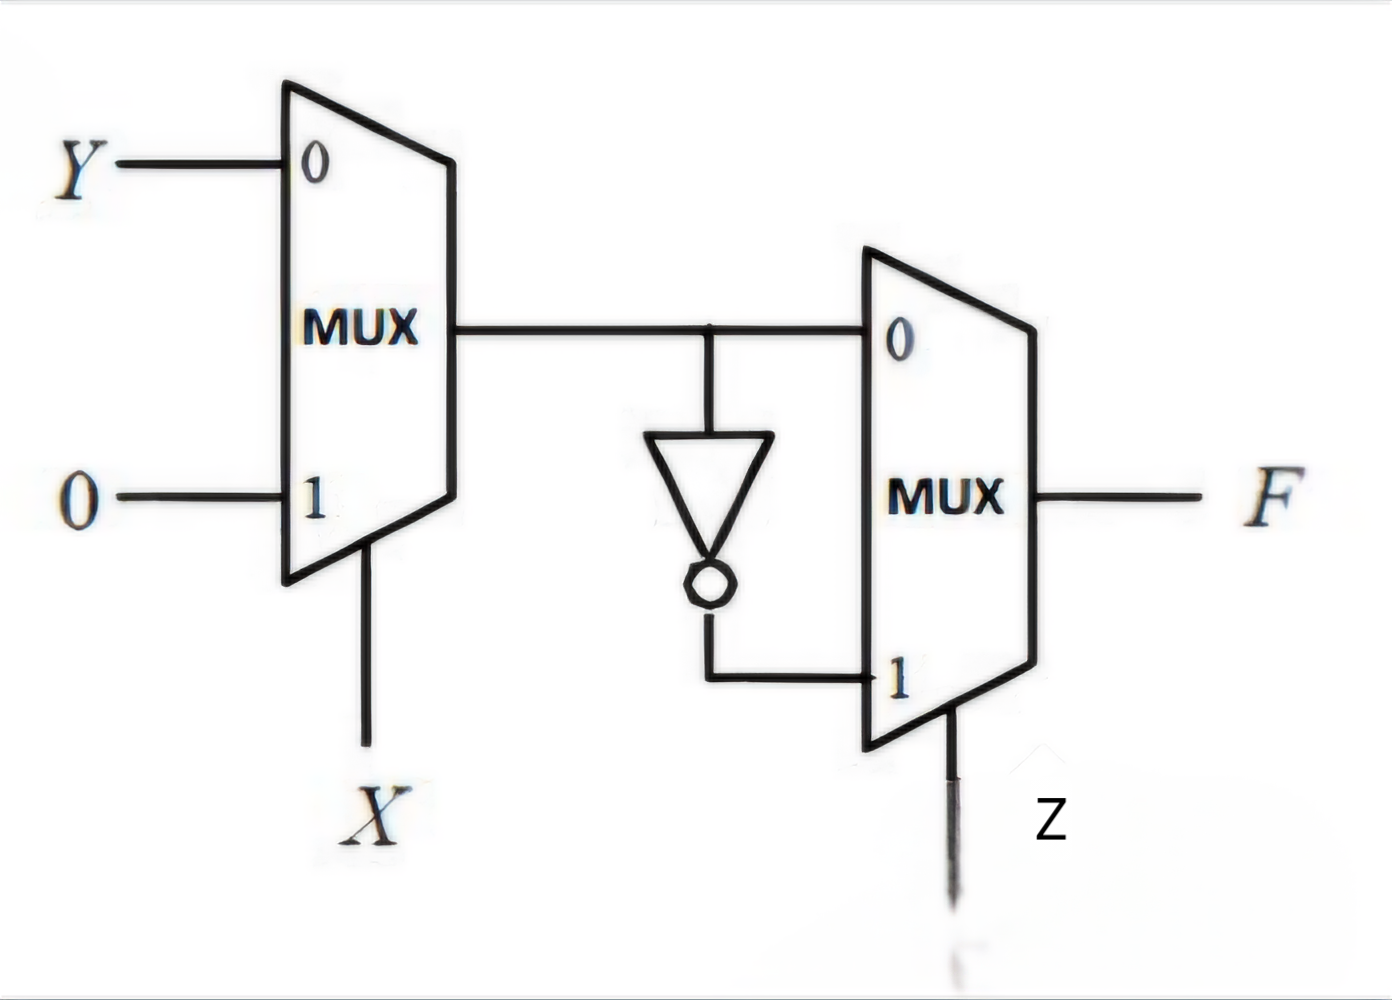
\includegraphics[width=0.5\columnwidth]{figs/2017-gate-ec-16.png}
\caption{}
\label{fig:2017-gate-ec-16}
\end{figure}
\item A Boolean digital circuit is composed using two 4-input multiplexers $M1$ and $M2$ and one 2-input multiplexer $M3$ as shown in the 
    \figref{fig:Multiplexer}.
	 $X0$–$X7$ are the inputs of the multiplexers $M1$ and $M2$ and could be connected to either $0$ or $1$. The select lines of the multiplexers are connected to Boolean variables $A$, $B$ and $C$ as shown.
Which one of the following set of values of $(X0, X1, X2, X3, X4, X5, X6, X7)$ will realise the Boolean function 
$\overline{A} + \overline{A}\overline{C}+A\overline{B}C $ ?
\hfill(GATE CS 2023)
 \begin{enumerate}
     \item (1, 1, 0, 0, 1, 1, 1, 0)
     \item (1, 1, 0, 0, 1, 1, 0, 1)
     \item (1, 1, 0, 1, 1, 1, 0, 0)
     \item (0, 0, 1, 1, 0, 1, 1, 1)
 \end{enumerate}
%
\begin{figure}[H]
    \centering
        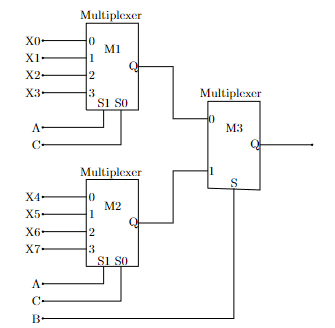
\includegraphics[width=0.75\columnwidth]{figs/Multiplexer.png}
    \caption{Digital Circuit}
    \label{fig:Multiplexer}
\end{figure}
%
\item Consider the boolean Function $z\brak{a,b,c}$ from 
			\figref{fig:203} below.
		Which of the following minterm lists represent the circuit given above?
	\begin{enumerate}
		\item $z=\Sigma\brak{0,1,3,7}$
		\item $z=\Sigma\brak{1,4,5,6,7}$
		\item $z=\Sigma\brak{2,4,5,6,7}$
		\item $z=\Sigma\brak{2,3,5}$
	\end{enumerate}	   
	\hfill{(GATE CS 2020)}
%	
		\begin{figure}[H]
			\centering
			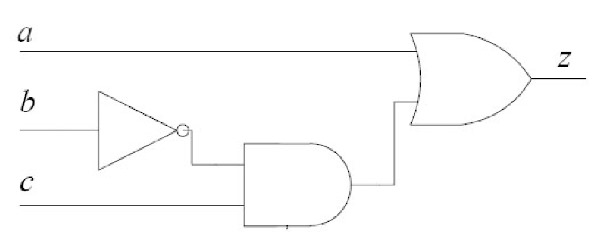
\includegraphics[width=0.5\columnwidth]{figs/203.png}
			\caption{}
			\label{fig:203}
		\end{figure}
%
\item Consider three $4$-variable functions $f_1, f_2, $and $f_3,$ which are expressed in sum-of-minterms as 
$$f_1 = \sum\brak{0,2,5,8,14}, f_2=\sum\brak{2,3,6,8,14,15}, f_3 = \sum\brak{2,7,11,14}.$$ For the following circuit 
	in 
	\figref{fig:GATE-CS2019,30},
	with one AND gate and one XOR gate, the output function $f$ can be expressed as
		\begin{enumerate}
		\item $\sum\brak{7,8,11}$
		\item $\sum\brak{2,7,8,11,14}$
		\item $\sum\brak{2,14}$
		\item $\sum\brak{0,2,3,5,6,7,8,11,14,15}$
		\end{enumerate}
%
	\hfill(GATE CS 2019)
	\begin{figure}[H]
		 \centering
		 \resizebox{0.5\columnwidth}{!}{%
			\begin{circuitikz}
    % Draw AND gate
    \draw (0,0) node[and port] (and) {AND};
    
    % Draw XOR gate
    \draw (4,-0.2) node[xor port] (xor) {XOR};
    
    % Connect AND output to XOR input
    \draw (and.out) -- (xor.in 1);
    
    % Draw input wires
    \draw (and.in 1) -- ++(-1,0) node[left] {$f_1$};
    \draw (and.in 2) -- ++(-1,0) node[left] {$f_2$};
    \draw (xor.in 2)--++(-90:2) --++(-5,0) node[left] {$f_3$};    % Draw XOR output
    \draw (xor.out) -- ++(1,0) node[right] {$f$};
\end{circuitikz}


			}
                 \caption{}
	\label{fig:GATE-CS2019,30}
	\end{figure}
\item For the logic circuit shown in \figref{fig:2000/gate/ec/2/7}, find the simplified Boolean expression for the output. 
\label{prob:2000/gate/ec/2/7}
\hfill (GATE EC 2000)
\begin{figure}[H]
    \centering
    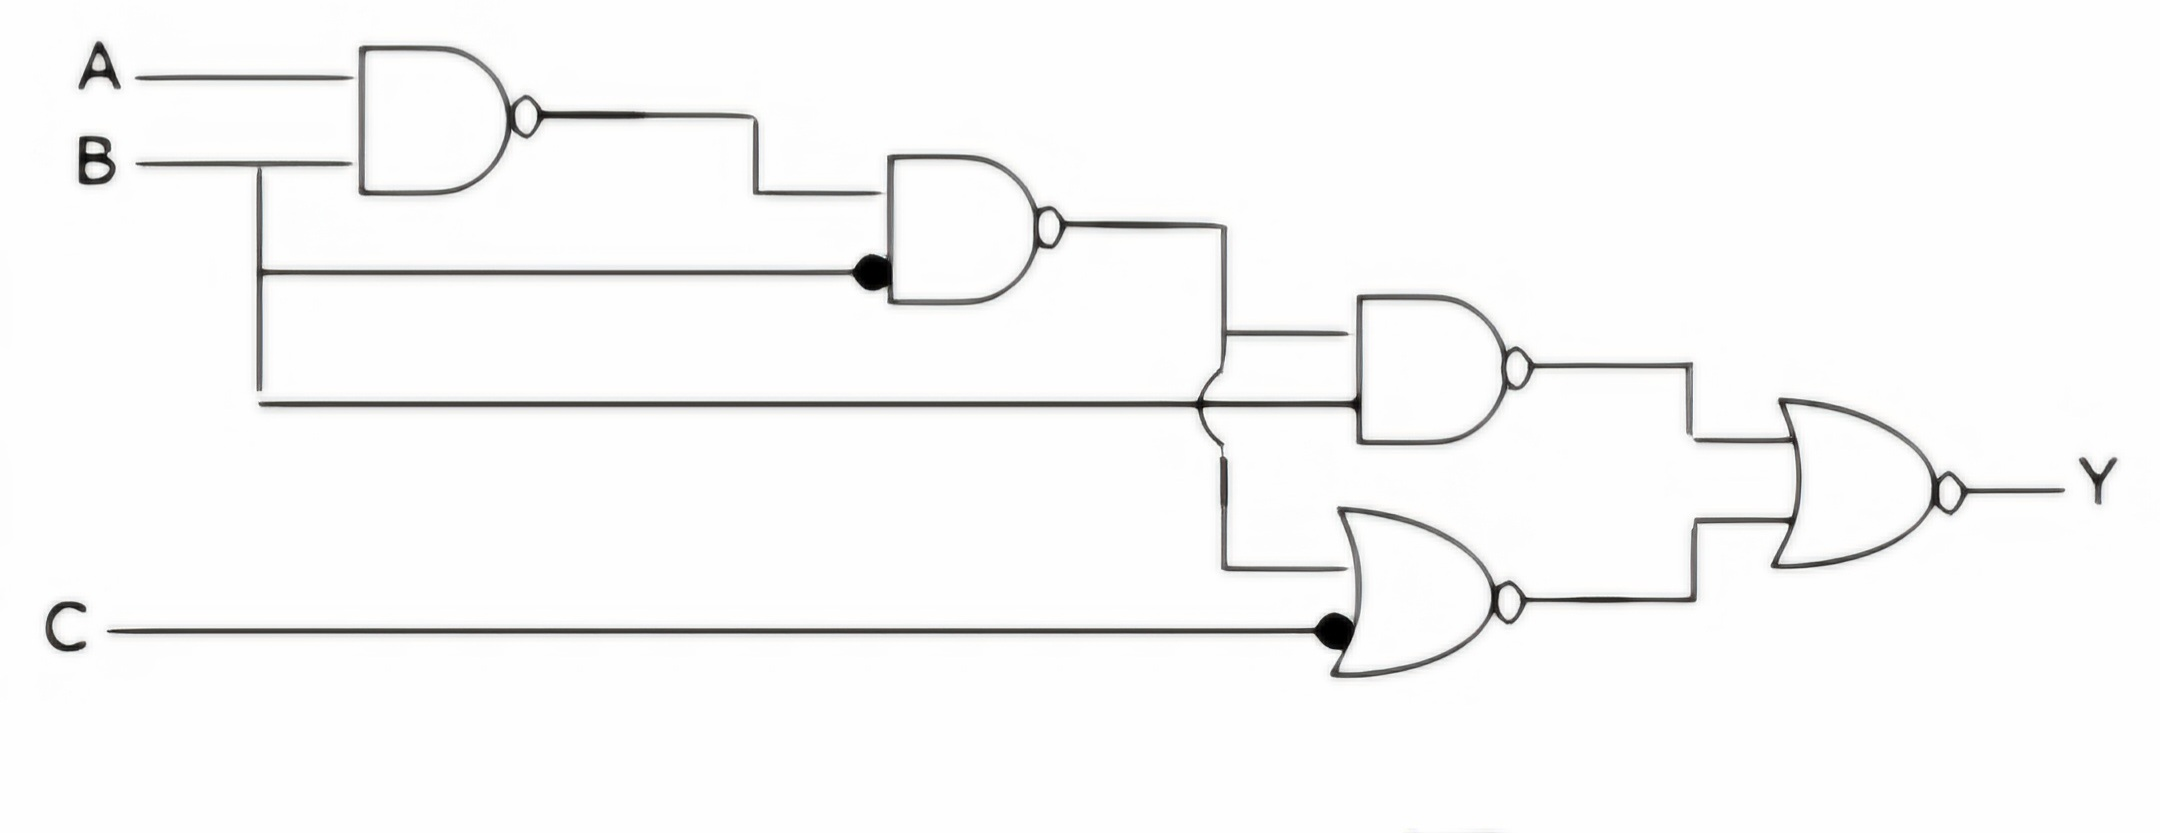
\includegraphics[width=0.75\columnwidth]{figs/2000-gate-ec-2-7.jpg}
    \caption{}
\label{fig:2000/gate/ec/2/7}
\end{figure}
\item Consider the Boolean function Z\brak{a,b,c}. Which one of the following minterm lists represents the 
 circuit given below  
 in
	 \figref{fig:GATE CS 2020}?
 \begin{figure}[H]
	 \centering
	 \resizebox{0.75\columnwidth}{!}{%
\begin{circuitikz}
    % Input nodes
    \node (a) at (0,-0.15) {$a$};
    \node (b) at (0,-1) {$b$};
    \node (c) at (0,-3) {$c$};

    % NOT gate
    \node [not port] at (2,-1) (not) {};
    \draw (b) -- (not.in);

    % AND gate
    \node [and port] at (5,-2.75) (and) {};
    \draw (not.out) -| (and.in 1);
    \draw (c) -- (and.in 2);

    % OR gate
    \node [or port] at (8,-0.45) (or) {};
    \draw (a) -- (or.in 1);
    \draw (and.out) -| (or.in 2);

    % Output
    \node (z) at (9,-0.5) {$z$};
    \draw (or.out) -- (z);
\end{circuitikz}

	 }
	 \caption{}
	 \label{fig:GATE CS 2020}
 \end{figure}
\begin{enumerate}[label=\Alph*.]
 \item $z=\sum{\brak{0,1,3,7}}$
 \item $z=\sum{\brak{1,4,5,6,7}}$
 \item $z=\sum{\brak{2,4,5,6,7}}$
 \item $z=\sum{\brak{2,3,5}}$
\end{enumerate}
\hfill (GATE CS 2020)
 \item The Boolean expression $F\brak{X,Y,Z} = \overline{X}Y\overline{Z}+X\overline{Y}\overline{Z}+XY\overline{Z}+XYZ$ converted into the canonical product of sum (POS) form is
 \begin{enumerate}
     \item $\brak{X+Y+Z}\brak{X+Y+\overline{Z}}\brak{X+\overline{Y}+\overline{Z}}\brak{\overline{X}+Y+\overline{Z}}$
     \item $\brak{X+\overline{Y}+Z}\brak{\overline{X}+Y+\overline{Z}}\brak{\overline{X}+\overline{Y}+Z}\brak{\overline{X}+\overline{Y}+\overline{Z}}$
     \item $\brak{X+Y+Z}\brak{\overline{X}+Y+\overline{Z}}\brak{X+\overline{Y}+Z}\brak{\overline{X}+\overline{Y}+\overline{Z}}$
     \item $\brak{X+\overline{Y}+\overline{Z}}\brak{\overline{X}+Y+Z}\brak{\overline{X}+\overline{Y}+Z}\brak{X+Y+Z}$
 \end{enumerate}
\hfill (GATE EC 2015)
\item
	 Consider the $2$-bit multiplexer (MUX) shown in  
		 \figref{fig:MUX}.
	  For OUTPUT to be the XOR of C and D, the values for $A_0,A_1,A_2$ and $A_3$  are  \rule{1cm}{0.1pt}. \hfill(GATE EC 2022)
	 \begin{enumerate}
		\item $A_0=0,A_1=0,A_2=1,A_3=1$
		\item $A_0=1,A_1=0,A_2=1,A_3=0$
		\item $A_0=0,A_1=1,A_2=1,A_3=0$
		\item $A_0=1,A_1=1,A_2=0,A_3=0$
	\end{enumerate}
	 \begin{figure}[H]
		 \centering
		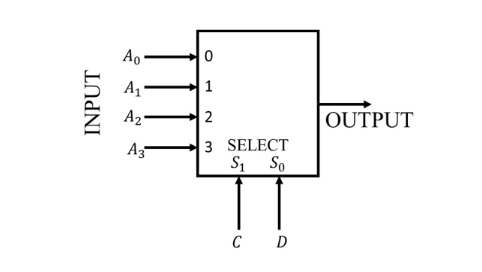
\includegraphics[width=0.5\columnwidth]{figs/gatepic19.jpg}
		\caption{MUX}
		 \label{fig:MUX}
	\end{figure}

\end{enumerate}




